\documentclass{article}


% if you need to pass options to natbib, use, e.g.:
%     \PassOptionsToPackage{numbers, compress}{natbib}
% before loading neurips_2023


% ready for submission
\usepackage[preprint]{neurips_2023}


% to compile a preprint version, e.g., for submission to arXiv, add add the
% [preprint] option:
%     \usepackage[preprint]{neurips_2023}


% to compile a camera-ready version, add the [final] option, e.g.:
%     \usepackage[final]{neurips_2023}


% to avoid loading the natbib package, add option nonatbib:
%    \usepackage[nonatbib]{neurips_2023}


\usepackage[utf8]{inputenc} % allow utf-8 input
\usepackage[T1]{fontenc}    % use 8-bit T1 fonts
\usepackage{hyperref}       % hyperlinks
\usepackage{url}            % simple URL typesetting
\usepackage{booktabs}       % professional-quality tables
\usepackage{amsfonts}       % blackboard math symbols
\usepackage{nicefrac}       % compact symbols for 1/2, etc.
\usepackage{microtype}      % microtypography
\usepackage{xcolor}
\usepackage{amsmath}         % colors
\usepackage{tikz}
\usetikzlibrary{backgrounds, positioning, fit}

\title{Distributed Databases Project}


% The \author macro works with any number of authors. There are two commands
% used to separate the names and addresses of multiple authors: \And and \AND.
%
% Using \And between authors leaves it to LaTeX to determine where to break the
% lines. Using \AND forces a line break at that point. So, if LaTeX puts 3 of 4
% authors names on the first line, and the last on the second line, try using
% \AND instead of \And before the third author name.


\author{
    Jop Zitman 2023280072\\
    Department of Computer Science\\
    Tsinghua University\\
    Beijing, China \\
    \texttt{zitmanj10@mails.tsinghua.edu.cn}
    \And
    Borislav Pavlov\\
    Department of Computer Science\\
    Tsinghua University\\
    \texttt{}
}


\begin{document}

    \maketitle

    \begin{abstract}
        % TODO: Compose a concise abstract summarizing the document's content.
    \end{abstract}


    \section{Introduction and Motivation}
    The advent of distributed systems has revolutionized the way data is stored, accessed, and processed. As the digital universe expands exponentially, there is an incessant demand for systems that can handle vast and varied data types efficiently. This project seeks to address these needs by developing a distributed database system tailored to manage an extensive array of articles and user interactions. The envisioned system is not only required to handle high volumes of both structured and unstructured data but also ensure that data retrieval is both swift and reliable, accommodating a significant number of concurrent users. Furthermore, the system's architecture should be robust enough to maintain functionality even in the face of certain system failures, thereby ensuring a degree of fault tolerance crucial for maintaining service continuity.

    Achieving this ambitious set of objectives necessitates a multifaceted approach involving the development of a scalable API server for data access, the integration of structured and unstructured data stores, the implementation of effective caching mechanisms to expedite data retrieval, and a comprehensive solution for monitoring system components to guarantee optimal performance and reliability.

    This project is not just an academic exercise; it is a vital step towards understanding and leveraging cutting-edge big data management techniques, with profound implications for real-world applications. By dissecting and reconstructing the complexities of distributed databases, we aim to contribute meaningfully to the field's body of knowledge and pave the way for innovative solutions to data management challenges.


    \section{Literature Review}
    %TODO: Provide an overview of existing distributed database systems, highlighting their limitations and areas for improvement. Discuss the evolution of database technologies, from traditional relational databases to NoSQL and NewSQL systems, and the varying approaches to handling big data challenges.


    \section{Problem Statement}
    Central to our investigation is a meticulously generated dataset, which includes a wide variety of article contents such as texts, images, and videos. The system's capability to handle and process this data is contingent upon several foundational tables, each serving a distinct but interconnected function:

    \begin{itemize}
        \item \textbf{User}: This table is essential for capturing personal information about users, delineated by regional demographics. By understanding user profiles, the system can provide tailored content and improve user experience.
        \item \textbf{Article}: Articles form the core of the content being managed. This table stores details about the articles, organized by categories, facilitating efficient retrieval and management of content.
        \item \textbf{Read}: Capturing how users interact with articles over time, this table is pivotal for understanding user engagement and preferences, informing content strategy and system optimizations.
        \item \textbf{Be-Read}: As an aggregate of the \textbf{Read} table, it reflects comprehensive readership metrics, including readership counts, agreements, and shares, indexed by article category. This data is vital for understanding content popularity and user interaction trends.
        \item \textbf{Popular-Rank}: This table synthesizes interaction data to rank content according to various metrics, providing insights into what is trending or valuable to different user segments.
    \end{itemize}

    These components, while individually significant, collectively contribute to a robust and dynamic system capable of adapting to and evolving with the needs of its users. The system must not only store and manage this data efficiently but also derive actionable insights to continuously enhance user experience and system performance.

    %TODO: Elaborate on the technical and practical challenges involved in managing and processing such a dataset.


    \section{Proposed Methodology}
    To construct a system that meets our ambitious goals, we propose an integrated solution comprising several cutting-edge technologies, each selected for its proven efficacy and relevance to the project's objectives. We will first discuss the rationale behind our technology choices and then elaborate on how these technologies will be integrated to create our system.


    \subsection{Technology Choices}

    \subsubsection{Containerization with Docker}
    Docker's containerization technology is foundational to ensuring that our application is portable, consistent, and isolated from environmental inconsistencies across development and production platforms. This modularity is critical for testing, deployment, and scaling, allowing each component of the system to be developed, deployed, and scaled independently.

    Docker utilizes Linux containers to package applications and their dependencies into isolated, executable components, reducing the overhead of creating and maintaining full virtual machines for running applications. It provides a toolkit for developers to build, deploy, and run containers using basic commands and automation, ensuring consistent environments across various stages of the development lifecycle.

    The adaptability of Docker's containerization supports responsive deployment and scaling. Docker containers can be executed in diverse environments, from a developer's local laptop to various cloud providers, emphasizing the need for efficient deployment and management across different platforms.

    Launched in 2013 as an open-source Docker Engine, Docker leveraged existing computing concepts around containers, particularly in the Linux world, using primitives known as cgroups and namespaces. This standardization has made the complex concepts of containerization more accessible and efficient for contemporary development needs.

    Docker's emergence has significantly accelerated the adoption of containerization technology. By abstracting complex containerization concepts into a user-friendly format, it has become an industry standard for containers, offering simple developer tools and a universal packaging approach. The widespread adoption of Docker underscores its importance as a tool for modern software development, testing, deployment, and scaling.

    \subsubsection{Orchestration with Kubernetes}
    Kubernetes stands at the forefront of container orchestration technologies, automating various manual processes related to managing containers such as scheduling, launching, scaling, and healing. It is capable of handling multiple groups of containers across more than one cluster simultaneously, providing essential features like service discovery, load balancing, storage orchestration, and maintaining environmental consistency throughout different stages of development. Built on a set of loosely coupled, extensible building blocks (primitives) that rely on the Kubernetes API, Kubernetes introduces a robust, portable, and extensible open-source platform for managing containerized workloads and services, facilitating both declarative configuration and automation.

    Also known as K8s, Kubernetes orchestrates the deployment, scaling, and management of containerized applications, grouping them into logical units for easy management and discovery. This system significantly enhances the orchestration of containerized applications across a cluster of nodes, which includes networking and storage infrastructure. One of its key features is resource scheduling, ensuring optimal distribution of Pods across all available nodes to maintain efficiency and balance.

    Among its notable features is automatic bin packing, where Kubernetes intelligently positions containers based on required resources and other constraints, without compromising availability. This sophisticated resource management capability allows Kubernetes to automatically specify how each container in a pod consumes resources like CPU and RAM, further ensuring that applications run smoothly and efficiently.

    Kubernetes' extensive ecosystem and its ability to streamline deployment, scaling, and operations of application containers render it an indispensable tool for automating and managing the lifecycle of containerized applications, ensuring the system's reliability and scalability.

    \subsubsection{Package Management with Helm Charts}
    Helm enhances Kubernetes's capabilities by facilitating the definition, installation, and upgrade of even the most complex Kubernetes applications. As an official Kubernetes deployment tool and part of the Cloud Native Computing Foundation, Helm simplifies the management of creation, packaging, configuration, and deployment of applications and services to Kubernetes clusters through Helm Charts. These charts are collections of Kubernetes YAML files designed to simplify the deployment process, making Helm an essential tool for modern application management in Kubernetes environments.

    Helm Charts are created and maintained by a range of contributors including individual developers, organizations, cloud service providers, and technology vendors. Among these, Bitnami is a prominent contributor, offering a wide range of pre-packaged, production-ready Helm charts for various applications. These charts are known for their quality and reliability, ensuring that applications deployed using Bitnami’s charts meet high standards of security and performance.

    As a package manager specifically for Kubernetes, Helm allows developers and operators to more easily package, configure, and deploy applications and services onto Kubernetes clusters. It addresses the need for managing the complexity and lifecycle of applications and their components, streamlining installation and updating processes, and maintaining a historical versioning of deployed applications.

    Helm's ability to automate YAML manifests for Kubernetes objects and package information into charts makes it an invaluable tool for deploying to a Kubernetes cluster. It also tracks the versioned history of each chart installation and change, enabling comprehensible commands to roll back to a previous version or upgrade to a newer one, thus maintaining consistency and reliability in deployments.

    Overall, Helm significantly contributes to the Kubernetes ecosystem by offering a streamlined, efficient method for package management, ultimately enhancing the scalability and management of containerized applications. Its wide adoption and support from various contributors, especially Bitnami, underline the collaborative and community-driven approach in managing and deploying applications in containerized environments.

    \subsubsection{Unstructured Data Management with MinIO}
    MinIO offers an efficient and scalable solution for managing unstructured data with its high-performance, S3 compatible object storage system. It is Kubernetes-native, providing a consistent object storage interface across multiple cloud providers, on-premise, and at the edge. As the world's fastest object store, MinIO delivers exceptional performance with published GETs and PUTs results that exceed 325 GiB/sec and 165 GiB/sec on 32 nodes of NVMe drives and a 100Gbe network, offering a portable and high-performance storage system across all major Kubernetes platforms. It is widely trusted and utilized by multiple organizations for its performance and reliability.

    MinIO is recommended for complete S3 API functionality for object storage on Kubernetes, providing a single global namespace and a consistent object storage interface across various environments. Its cloud-native and lightweight architecture allows it to run efficiently on low CPU and memory resources, enabling the hosting of a large number of tenants on shared hardware. This makes MinIO particularly effective in environments where resource efficiency and scalability are crucial.

    MinIO's object storage solution supports all core S3 features and is built to deploy anywhere, from public or private clouds to bare metal infrastructure, orchestrated environments, and edge infrastructure. This versatility ensures that MinIO can cater to the varied and dynamic storage needs of modern applications and systems.

    In summary, MinIO's high performance, robust fault tolerance mechanisms like erasure coding, and compatibility with a variety of cloud storage services make it a crucial component for managing unstructured data in containerized environments. Its integration with Kubernetes through the MinIO Operator enhances its capability to provide reliable and scalable object storage solutions, addressing the complex and varied data management needs of contemporary systems.

    \subsubsection{Structured Data Handling with MongoDB}
    MongoDB's flexible, document-oriented structure makes it particularly adept at managing structured data in our system. Its scalability, powerful indexing and querying capabilities, and support for complex aggregations and transactions ensure that our structured data is handled efficiently and effectively. Running MongoDB on Kubernetes requires careful consideration of storage options and proper configuration to optimize performance and reliability. The Bitnami Helm chart is a popular, well-documented option for deploying MongoDB, offering various configurations like standalone, replica set, or replica set with arbiter, simplifying the deployment and management of MongoDB within Kubernetes.

    \subsubsection{Caching with Redis}
    Redis will serve as our primary caching solution in the Kubernetes environment, significantly enhancing the system's performance by reducing the load on databases and accelerating data retrieval. Redis's versatility in configurations and renowned performance makes it an ideal choice for caching needs. Its integration with Kubernetes ensures scalable and efficient management of cache instances, further optimizing the performance and responsiveness of applications.

    \subsubsection{API Development with FastAPI}
    FastAPI is an excellent choice for projects involving Kubernetes, Redis, MongoDB, and S3 due to its high performance, asynchronous support, and ease of use. As one of the fastest web frameworks for Python, it can efficiently handle high-load scenarios and large numbers of concurrent users, essential for systems utilizing databases like MongoDB and caching mechanisms like Redis. Its asynchronous handling is particularly beneficial for IO-bound tasks, common with interactions in MongoDB, Redis, and S3. FastAPI's automatic data validation ensures robust integration, while its compatibility with Kubernetes makes it ideal for scalable, containerized applications. The framework's straightforward design, complete with automatic API documentation, significantly eases the development and management of complex services. Thus, FastAPI stands out as a robust, efficient, and developer-friendly option for building APIs in demanding and dynamic environments.

    \subsubsection{Monitoring}
    In a distributed system project, monitoring plays a crucial role in ensuring the performance and reliability of services. Monitoring is the real-time collection of metrics and logs from a system, providing insights into its health and performance. It is essential for maintaining system stability and efficiency, allowing operators to identify and resolve issues before they impact users. Centralized monitoring is particularly important in distributed systems, where the complexity of the system and the number of components make it difficult to identify and resolve issues without proper monitoring.

    \textbf{Metrics}:
    Prometheus is a key tool in this domain, serving as an open-source monitoring and alerting toolkit with a powerful time-series database and query language. For this project, we decided to use Prometheus as a metrics scraping platform due to its popularity, ease of use, and compatibility with Kubernetes and many other open-source applications (many projects provide prometheus metrics endpoints).

    \textbf{Logging}:
    Logging allows for the collection of events and messages from a system, providing a record of its activity, such as errors or informational messages. It is crucial for monitoring and troubleshooting, allowing operators to identify and resolve issues. Loki is an open-source, horizontally scalable, highly available log aggregation system inspired by Prometheus. It is designed to be cost-effective and easy to operate, using labels to organize log streams and queries to filter log streams, making it highly efficient and scalable. Unfortunately, we no longer had time to properly test and debug the Loki deployment, so we have omitted it from this project.

    \textbf{Alerting}:
    Alerting is a crucial component of monitoring, allowing operators to be notified of issues and resolve them before they impact users. AlertManager is an open-source alerting system that works with Prometheus to send alerts to various receivers, including email, Slack, and more. It allows for the grouping and deduplication of alerts, ensuring that operators are not overwhelmed by a flood of alerts. AlertManager is highly configurable, allowing for the creation of complex alerting rules and routing trees, making it a powerful tool for monitoring and alerting.

    \textbf{Dashboarding}:
    The facto choice for dashboard management in the Prometheus ecosystem is Grafana, an open-source visualization platform that allows users to create, explore, and share dashboards that visualize the metrics data collected by Prometheus. Grafana is highly customizable, with a wide range of plugins and community-built dashboards, making it an ideal choice for monitoring and visualization. It also integrates with AlertManager, allowing for the creation of dashboards that display alerts and their status.

    \textbf{Prometheus Operator}
    These tools are deployed using the Prometheus Operator, a method that simplifies the deployment and management of Prometheus, Grafana, and Alertmanager in Kubernetes environments. The operator provides a cluster-wide framework for lifecycle management, including resource deployment and configuration, and offers a more automated and scalable approach to monitoring. Within this setup, the new K8s objects ServiceMonitors and PodMonitors are crucial. ServiceMonitors define how groups of services should be monitored by Prometheus, specifying the endpoints to scrape metrics from, along with the scraping interval and other parameters. They are particularly useful for monitoring services that dynamically scale within Kubernetes. On the other hand, PodMonitors offer a more granular approach by allowing Prometheus to scrape metrics from specific pods, giving insights into the performance of individual pods outside the service abstraction. Many Bitnami Helm charts provide ServiceMonitors and PodMonitors out of the box, making them an ideal choice for monitoring.

    Together, Prometheus, Grafana, and AlertManager, when deployed via the Prometheus Operator and utilizing ServiceMonitors and PodMonitors, create a powerful, scalable monitoring solution that can adapt to the changing landscape of a distributed system, providing vital metrics and alerts to maintain system health and performance.

    \subsection{System Architecture}
    This section provides an overview of the deployment and interaction of various components within the system. Our architecture is designed for scalability, high availability, and robust monitoring, utilizing a combination of Kubernetes, databases, storage solutions, and a Python API.

    \subsection{Deployment Overview}

    \begin{itemize}
        \item \textbf{Kubernetes on Minikube:} Minikube is used to deploy a Kubernetes cluster on a local machine. This will allow us to test and develop our system in a local environment before deploying it to a cloud provider.
        \item \textbf{Monitoring Tools:} Prometheus operator with default Grafana and Alertmanager.
        \item \textbf{Minio S3 Storage:} Default MinIO provided chart configured with 4 nodes, each with 2 drives, and service-monitors for Prometheus.
        \item \textbf{MongoDB:} Bitnami provided chart configured with a cluster of 3 config servers, 3 mongos routers, and 2 shards, each with 3 replicas. It includes prometheus pod monitors too.
        \item \textbf{Redis:} Deployed with 1 master and 3 replicas without persistence and with service and pod monitors included.
        \item \textbf{API:} Simple K8s service and deployment with 3 replicas.
    \end{itemize}

    \subsection{Component Interaction}

    Components in the system interact as follows:

    \begin{itemize}
        \item Kubernetes orchestrates all components, managing their lifecycle, scaling, and networking.
        \item The Python API interacts with Minio for object storage, MongoDB for persistent data storage, and Redis for caching.
        \item Monitoring tools are integrated throughout, with Prometheus gathering metrics, Grafana for visualization, and Alertmanager handling alerts.
    \end{itemize}
    \subsection{Architecture Diagram}
    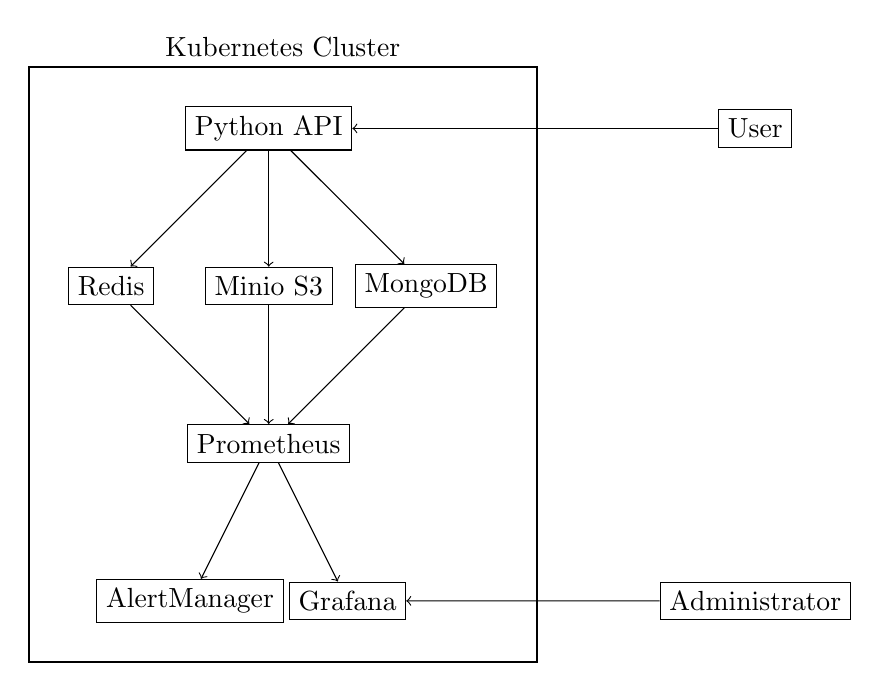
\begin{tikzpicture}[node distance=2cm]
        \node (python) [draw] {Python API};
        \node (mongo) [below of=python, xshift=2cm, draw] {MongoDB};
        \node (redis) [below of=python, xshift=-2cm, draw] {Redis};
        \node (minio) [below of=python, draw] {Minio S3};

        \node (prometheus) [below of=minio, draw] {Prometheus};
        \node (grafana) [below of=prometheus, xshift=1cm, draw] {Grafana};
        \node (alert) [below of=prometheus, xshift=-1cm, draw] {AlertManager};


        % Lines
        \draw [->] (python) -- (minio);
        \draw [->] (python) -- (redis);
        \draw [->] (python) -- (mongo);
        \draw [->] (minio) -- (prometheus);
        \draw [->] (mongo) -- (prometheus);
        \draw [->] (redis) -- (prometheus);
        \draw [->] (prometheus) -- (grafana);
        \draw [->] (prometheus) -- (alert);

        \begin{scope}[on background layer]
            \node (kubernetes) [draw, thick, fit=(python) (mongo) (redis) (minio) (prometheus) (grafana) (alert), inner sep=0.5cm, label=above:Kubernetes Cluster] {};
        \end{scope}

        \node (user) [right of=kubernetes, xshift=4cm, yshift=3cm, draw] {User};
        \node (admin) [right of=kubernetes, xshift=4cm, yshift=-3cm, draw] {Administrator};

        \draw [->] (user) -- (python);
        \draw [->] (admin) -- (grafana);

    \end{tikzpicture}

    \subsection{Application Configuration}

    \subsubsection{MongoDB}


    %TODO: Delve deeper into how these technologies interrelate and collectively contribute to a cohesive, scalable, and efficient system.

    \section{Evaluation and Metrics}
    %TODO: Define the performance, scalability, and fault tolerance metrics. Discuss the evaluation methods, including simulation, real-world testing, and user feedback.


    \section{Conclusion}
    %TODO: Summarize the project's objectives, methodologies, and anticipated contributions to the field of distributed databases. Reflect on the implications of the project for future research and applications.

\end{document}

